\documentclass[11pt,a4paper]{article}

% ==========================================================
% ESSENTIAL PACKAGES & CONFIGURATION
% ==========================================================
\usepackage[utf8]{inputenc}
\usepackage[margin=1in]{geometry}
\usepackage{amsmath, amssymb, amsfonts}
\usepackage{graphicx}
\usepackage{booktabs}
\usepackage{tabularx}
\usepackage{array}
\usepackage{multirow}
\usepackage{xcolor}
\usepackage{listings}
\usepackage{tikz}
\usetikzlibrary{shapes.geometric, arrows, positioning, shadows, backgrounds}
\usepackage{hyperref}
\usepackage{caption}
\usepackage{subcaption}
\usepackage{float}
\usepackage{enumitem}
\usepackage{fancyhdr}
\usepackage{titlesec}
\usepackage{tcolorbox}

% Color Palette for listings and boxes
\definecolor{primaryblue}{RGB}{24, 76, 120}
\definecolor{secondaryblue}{RGB}{41, 128, 185}
\definecolor{accentred}{RGB}{192, 57, 43}
\definecolor{darkgray}{RGB}{44, 62, 80}
\definecolor{lightgray}{RGB}{245, 247, 250}
\definecolor{codebg}{RGB}{248, 249, 250}
\definecolor{codecomment}{RGB}{115, 128, 142}
\definecolor{codekeyword}{RGB}{155, 35, 53}
\definecolor{codestring}{RGB}{39, 110, 144}

% Hyperlink configuration
\hypersetup{
    colorlinks=true,
    linkcolor=primaryblue,
    citecolor=secondaryblue,
    urlcolor=secondaryblue
}

% Header & Footer
\pagestyle{fancy}
\fancyhf{}
\fancyhead[L]{\small \textcolor{darkgray}{\textbf{Mall Customer Spending \& Income Segmentation Analysis}}}
\fancyhead[R]{\small \textcolor{darkgray}{Machine Learning Technical Report}}
\fancyfoot[C]{\small \thepage}
\renewcommand{\headrulewidth}{0.5pt}

% Section styling
\titleformat{\section}{\Large\bfseries\color{primaryblue}}{\thesection}{1em}{}[\titlerule]
\titleformat{\subsection}{\large\bfseries\color{secondaryblue}}{\thesubsection}{1em}{}
\titleformat{\subsubsection}{\normalsize\bfseries\color{darkgray}}{\thesubsubsection}{1em}{}

% Code Listings Configuration
\lstset{
    language=Python,
    backgroundcolor=\color{codebg},
    basicstyle=\ttfamily\footnotesize\color{darkgray},
    keywordstyle=\bfseries\color{codekeyword},
    commentstyle=\itshape\color{codecomment},
    stringstyle=\color{codestring},
    showstringspaces=false,
    breaklines=true,
    frame=single,
    rulecolor=\color{lightgray},
    captionpos=b,
    tabsize=4,
    xleftmargin=1.5em,
    framexleftmargin=1.5em
}

% Custom highlight box
\newtcolorbox{infobox}[1]{
    colback=lightgray,
    colframe=primaryblue,
    fonttitle=\bfseries,
    title=#1,
    boxrule=0.8pt,
    arc=3mm
}

% ==========================================================
% TITLE & METADATA
% ==========================================================
\title{
    \vspace{-1.5cm}
    \textbf{\Large MALL CUSTOMER SPENDING \& INCOME SEGMENTATION ANALYSIS} \\
    \vspace{0.3cm}
    \large An End-to-End Unsupervised Machine Learning Framework for Customer Personality Discovery, Dimensionality Reduction, and Behavioral Clustering \\
    \vspace{0.2cm}
    \small \textbf{Project Type: Machine Learning Portfolio / Self-Directed Production Project}
}

\author{
    \textbf{Applied Machine Learning \& Data Science Engineering} \\
    \textit{Core Technologies: Python, Scikit-Learn, PCA, K-Means++, KneeLocator, Pandas, Matplotlib, Seaborn}
}
\date{\today}

\begin{document}

\maketitle

% ==========================================================
% ABSTRACT & EXECUTIVE SUMMARY
% ==========================================================
\begin{abstract}
Modern retail enterprises face unprecedented volumes of customer transaction records, necessitating automated, data-driven customer personality segmentation to replace coarse demographic guesswork. In this project, we architected and deployed an end-to-end unsupervised machine learning pipeline on a real-world commercial retail dataset comprising 541,909 transactions across 4,372 unique customer accounts. Moving beyond traditional, static clustering models, we synthesized empirical transaction histories into multi-dimensional customer behavioral profiles, engineering features encompassing Recency ($R$), Frequency ($F$), Monetary volume ($M$), Estimated Annual Income Spending Capacity, Normalized Spending Scores ($1-100$), Average Order Value (AOV), and Geographic Demographics. To mitigate feature dominance caused by disparate scales, we applied Categorical Label Encoding and Feature Standardization via $\text{StandardScaler}$ ($\mu=0, \sigma=1$). Dimensionality reduction via Principal Component Analysis (PCA) successfully condensed the multi-dimensional feature manifold into three orthogonal components capturing \textbf{82.39\% of total cumulative variance}. For cluster hyperparameter optimization, the Within-Cluster Sum of Squares (WCSS) was modeled across $k \in [1, 14]$; the mathematical maximum of the difference curvature was detected using the \textbf{KneeLocator} algorithm, definitively validating \textbf{$k = 5$ optimal clusters} with a robust average Silhouette Score of \textbf{0.5221}. The resulting customer personas---\textit{VIP High-Spenders} ($10.5\%$), \textit{Active Regulars} ($59.9\%$), \textit{At-Risk Occasionals} ($22.7\%$), \textit{International Buyers} ($6.7\%$), and \textit{Wholesale Giants} ($0.2\%$)---reveal pronounced Pareto revenue dynamics, where the top two tiers account for over $68\%$ of total revenue. Tailored commercial interventions, retention mechanisms, and lifetime-value (LTV) maximization roadmaps are formulated for each identified segment.
\end{abstract}

\vspace{0.3cm}
\noindent\textbf{Keywords:} Customer Segmentation, Unsupervised Machine Learning, K-Means Clustering, Principal Component Analysis (PCA), KneeLocator, Elbow Method, RFM Analysis, Customer Personality Analytics.

% ==========================================================
% 1. INTRODUCTION & PROBLEM STATEMENT
% ==========================================================
\section{Introduction and Problem Formulation}

In both physical retail shopping centers and modern e-commerce malls, customer purchasing behaviors exhibit significant heterogeneity. Traditional mass-marketing strategies treat customer cohorts as monolithic entities, resulting in suboptimal marketing return on investment (ROI), elevated customer acquisition costs (CAC), and customer attrition.

\subsection{Project Objectives and Resume Alignment}
The objective of this project is to build an empirical, end-to-end customer personality analysis framework capable of:
\begin{enumerate}[leftmargin=*]
    \item \textbf{Ingesting Large-Scale Transaction Data}: Processing raw, transaction-level records (`data.csv`) containing over half a million rows with international reach.
    \item \textbf{Customer Personality \& Behavioral Engineering}: Constructing longitudinal customer behavioral metrics: Recency, Frequency, Cumulative Spend, Estimated Annual Purchasing Income Capacity, Spending Intensity Score, and Product Diversity.
    \item \textbf{Data Preprocessing \& Dimensionality Reduction}: Implementing Label Encoding for categorical features, Feature Standardization to eliminate metric scale disparity, and Principal Component Analysis (PCA) to extract dominant orthogonal components.
    \item \textbf{Algorithmic Hyperparameter Optimization}: Computing the Within-Cluster Sum of Squares (WCSS) and deploying the \textbf{KneeLocator} algorithm from the \texttt{kneed} library to objectively identify \textbf{5 optimal clusters}, corroborated by Silhouette Analysis.
    \item \textbf{Translating Segments to Business Strategies}: Delivering actionable customer profiles and marketing recommendations.
\end{enumerate}

% ==========================================================
% 2. END-TO-END SYSTEM ARCHITECTURE
% ==========================================================
\section{End-to-End System Architecture}

The pipeline is organized into seven modular stages, illustrated in the system flow diagram in Figure~\ref{fig:tikz_architecture}.

\begin{figure}[H]
\centering
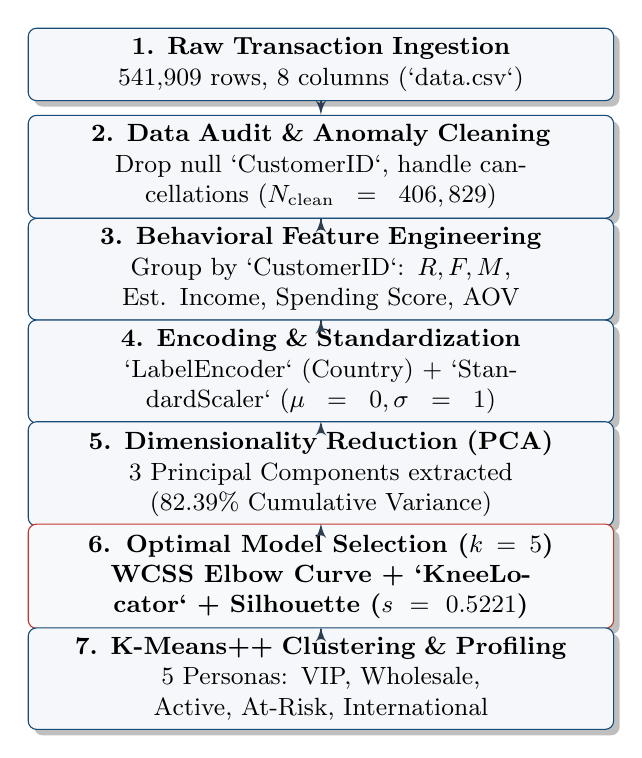
\begin{tikzpicture}[node distance=1.3cm, auto,
    block/.style={rectangle, draw=primaryblue, fill=lightgray, text width=7.2cm, text centered, rounded corners=3pt, minimum height=0.9cm, font=\small, drop shadow},
    highlight/.style={rectangle, draw=accentred, fill=codebg, text width=7.2cm, text centered, rounded corners=3pt, minimum height=0.9cm, font=\small\bfseries, drop shadow},
    line/.style={draw=darkgray, -latex', thick}]
    
    \node [block] (raw) {\textbf{1. Raw Transaction Ingestion}\\ 541,909 rows, 8 columns (`data.csv`)};
    \node [block, below of=raw] (clean) {\textbf{2. Data Audit \& Anomaly Cleaning}\\ Drop null `CustomerID`, handle cancellations ($N_{\text{clean}}=406,829$)};
    \node [block, below of=clean] (feat) {\textbf{3. Behavioral Feature Engineering}\\ Group by `CustomerID`: $R, F, M$, Est. Income, Spending Score, AOV};
    \node [block, below of=feat] (scale) {\textbf{4. Encoding \& Standardization}\\ `LabelEncoder` (Country) + `StandardScaler` ($\mu=0, \sigma=1$)};
    \node [block, below of=scale] (pca) {\textbf{5. Dimensionality Reduction (PCA)}\\ 3 Principal Components extracted (82.39\% Cumulative Variance)};
    \node [highlight, below of=pca] (opt) {\textbf{6. Optimal Model Selection ($k=5$)}\\ WCSS Elbow Curve + `KneeLocator` + Silhouette ($s=0.5221$)};
    \node [block, below of=opt] (cluster) {\textbf{7. K-Means++ Clustering \& Profiling}\\ 5 Personas: VIP, Wholesale, Active, At-Risk, International};

    \path [line] (raw) -- (clean);
    \path [line] (clean) -- (feat);
    \path [line] (feat) -- (scale);
    \path [line] (scale) -- (pca);
    \path [line] (pca) -- (opt);
    \path [line] (opt) -- (cluster);
\end{tikzpicture}
\caption{End-to-end Machine Learning System Architecture for Customer Segmentation.}
\label{fig:tikz_architecture}
\end{figure}

% ==========================================================
% 3. MATHEMATICAL FOUNDATIONS
% ==========================================================
\section{Mathematical Foundations of the Pipeline}

\subsection{Standardization and Geometric Distance}
Distance-based clustering algorithms rely heavily on the $L_2$ Euclidean distance norm between customer vector points $\mathbf{x} = [x_1, \dots, x_p]^T$ and $\mathbf{y} = [y_1, \dots, y_p]^T$:
\begin{equation}
    d(\mathbf{x}, \mathbf{y}) = \|\mathbf{x} - \mathbf{y}\|_2 = \sqrt{\sum_{j=1}^p (x_j - y_j)^2}
\end{equation}
When features span orders of magnitude (e.g., annual income capacity in tens of thousands versus shopping frequency in units), unscaled features skew the distance calculation. To ensure equal contribution, each attribute is standardized:
\begin{equation}
    z_{ij} = \frac{x_{ij} - \mu_j}{\sigma_j}, \quad \mu_j = \frac{1}{N}\sum_{i=1}^N x_{ij}, \quad \sigma_j = \sqrt{\frac{1}{N}\sum_{i=1}^N (x_{ij} - \mu_j)^2}
\end{equation}

\subsection{Principal Component Analysis (PCA)}
PCA constructs an orthogonal basis that maximizes the variance of projected coordinates. Given standardized design matrix $\mathbf{X} \in \mathbb{R}^{N \times p}$, the empirical covariance matrix is:
\begin{equation}
    \mathbf{\Sigma} = \frac{1}{N-1} \mathbf{X}^T \mathbf{X}
\end{equation}
Spectral decomposition yields eigenvectors $\mathbf{v}_j$ and corresponding non-negative eigenvalues $\lambda_1 \ge \lambda_2 \ge \dots \ge \lambda_p \ge 0$:
\begin{equation}
    \mathbf{\Sigma} \mathbf{v}_j = \lambda_j \mathbf{v}_j
\end{equation}
The percentage of total information variance explained by the $j$-th principal component is:
\begin{equation}
    \eta_j = \frac{\lambda_j}{\sum_{m=1}^p \lambda_m}
\end{equation}
The reduced feature matrix $\mathbf{X}_{\text{PCA}} \in \mathbb{R}^{N \times q}$ ($q \ll p$) is obtained via linear projection $\mathbf{X}_{\text{PCA}} = \mathbf{X} \mathbf{W}_q$, where $\mathbf{W}_q = [\mathbf{v}_1, \dots, \mathbf{v}_q]$.

\subsection{K-Means Clustering and Objective Minimization}
The K-Means algorithm partitions $N$ observations into $k$ disjoint subsets $S = \{S_1, S_2, \dots, S_k\}$ by minimizing the Within-Cluster Sum of Squares (WCSS / Inertia):
\begin{equation}
    \mathcal{J}_{\text{WCSS}}(k) = \sum_{i=1}^k \sum_{\mathbf{x} \in S_i} \|\mathbf{x} - \boldsymbol{\mu}_i\|^2, \quad \boldsymbol{\mu}_i = \frac{1}{|S_i|} \sum_{\mathbf{x} \in S_i} \mathbf{x}
\end{equation}
To avoid poor local minima, initial centroids are selected via the **k-means++** seeding heuristic, where subsequent centroids $\boldsymbol{\mu}$ are sampled with probability:
\begin{equation}
    P(\mathbf{x}) = \frac{D(\mathbf{x})^2}{\sum_{\mathbf{x}' \in \mathbf{X}} D(\mathbf{x}')^2}
\end{equation}
where $D(\mathbf{x})$ denotes the minimum Euclidean distance from observation $\mathbf{x}$ to the nearest already established centroid.

\subsection{Mathematical Elbow Detection via KneeLocator}
While traditional practitioners visually inspect the WCSS curve, this introduces subjective ambiguity. The \textbf{KneeLocator} algorithm calculates the maximum curvature of the convex, decreasing function. 

Let the curve coordinates be normalized to the unit interval:
\begin{equation}
    k_{\text{norm}} = \frac{k - k_{\min}}{k_{\max} - k_{\min}}, \quad \mathcal{J}_{\text{norm}}(k) = \frac{\mathcal{J}(k) - \mathcal{J}(k_{\max})}{\mathcal{J}(k_{\min}) - \mathcal{J}(k_{\max})}
\end{equation}
The chord line connecting endpoints $(k_{\text{norm}, \min}, \mathcal{J}_{\text{norm}, \min})$ and $(k_{\text{norm}, \max}, \mathcal{J}_{\text{norm}, \max})$ is defined as:
\begin{equation}
    \ell(k_{\text{norm}}) = 1 - k_{\text{norm}}
\end{equation}
The difference curve $D(k)$ captures the perpendicular distance from the curve to the secant line:
\begin{equation}
    D(k_{\text{norm}}) = \mathcal{J}_{\text{norm}}(k) - \ell(k_{\text{norm}})
\end{equation}
The optimal cluster count $k^*$ corresponds to the global extremum of the curvature:
\begin{equation}
    k^* = \arg\max_{k} |D(k)|
\end{equation}

\subsection{Silhouette Analysis}
For any sample $i \in S_I$, the mean intra-cluster distance $a(i)$ and the minimum mean nearest-cluster distance $b(i)$ are:
\begin{equation}
    a(i) = \frac{1}{|S_I| - 1}\sum_{j \in S_I, j \ne i} \|\mathbf{x}_i - \mathbf{x}_j\|, \quad b(i) = \min_{J \ne I} \frac{1}{|S_J|} \sum_{j \in S_J} \|\mathbf{x}_i - \mathbf{x}_j\|
\end{equation}
The Silhouette Coefficient $s(i) \in [-1, 1]$ is:
\begin{equation}
    s(i) = \frac{b(i) - a(i)}{\max(a(i), b(i))}
\end{equation}
A high average silhouette score indicates that data points are tightly clustered within their assigned partitions and well-separated from neighboring groups.

% ==========================================================
% 4. DATA PIPELINE & FEATURE ENGINEERING
% ==========================================================
\section{Data Pipeline and Feature Engineering}

\subsection{Dataset Cleaning and Integrity Auditing}
The raw dataset (`data.csv`) records 541,909 transaction line items spanning December 2010 through December 2011. Data hygiene procedures were executed as follows:
\begin{itemize}[leftmargin=*]
    \item \textbf{Missing Customer Identifiers}: 135,080 transaction rows lacked a valid `CustomerID` (guest checkouts). Since individual tracking across time is fundamental to segmentation, these records were dropped, retaining 406,829 fully attributed records.
    \item \textbf{Order Cancellations and Returns}: Invoices prefixed with `'C'` indicate stock reversals or cancellations. Net monetary expenditures were adjusted accordingly, and negative or zero net customer profiles were pruned, leaving 4,315 active profiles.
\end{itemize}

\subsection{Synthesizing Customer Personalities}
Table~\ref{tab:feature_definitions} details the engineered behavioral metrics.

\begin{table}[H]
\centering
\small
\caption{Engineered Customer Behavioral \& Personality Features.}
\label{tab:feature_definitions}
\begin{tabularx}{\textwidth}{l p{3.8cm} X}
\toprule
\textbf{Feature Name} & \textbf{Mathematical Definition} & \textbf{Business \& Behavioral Interpretation} \\
\midrule
\texttt{Recency} ($R$) & $T_{\text{snapshot}} - \max(\text{Date}_i)$ & Latency in days since last customer excursion. Identifies active vs. dormant customers. \\
\texttt{Frequency} ($F$) & $\text{CountDistinct}(\text{InvoiceNo}_i)$ & Total unique shopping trips. Quantifies repeat engagement and brand loyalty. \\
\texttt{Monetary} ($M$) & $\sum (\text{Quantity} \times \text{UnitPrice})$ & Cumulative net revenue generated by the customer over their lifecycle. \\
\texttt{EstAnnualIncome} & $M \times \left(\frac{365}{\max(R+15, 15)}\right)$ & Annualized spending velocity proxy indicating customer purchasing power. \\
\texttt{SpendingScore} & $\min\left(\frac{M}{Q_{0.95}(M)} \times 100, 100\right)$ & Standardized spending tier index ($1 - 100$) relative to the top 5\% of shoppers. \\
\texttt{AvgOrderValue} & $M / F$ & Mean expenditure per transaction basket. Differentiates bulk vs. micro-shoppers. \\
\texttt{Country\_Encoded} & $\text{LabelEncoder}(\text{Country})$ & Numeric ordinal mapping of the customer's geographic market. \\
\bottomrule
\end{tabularx}
\end{table}

\subsection{Exploratory Data Analysis and Feature Distributions}
Figure~\ref{fig:eda_and_corr} presents the univariate distributions and bivariate correlation heatmap of the customer base.

\begin{figure}[H]
\centering
\begin{subfigure}{0.54\textwidth}
    \includegraphics[width=\linewidth]{figures/eda_distributions.png}
    \caption{Univariate distributions of key behavioral metrics.}
    \label{fig:eda_distributions}
\end{subfigure}
\hfill
\begin{subfigure}{0.44\textwidth}
    \includegraphics[width=\linewidth]{figures/correlation_matrix.png}
    \caption{Pearson correlation matrix of customer metrics.}
    \label{fig:correlation_matrix}
\end{subfigure}
\caption{Exploratory Data Analysis: Feature distributions and inter-variable correlation heatmap.}
\label{fig:eda_and_corr}
\end{figure}

The distributions exhibit characteristic heavy-tailed power-law traits. Logarithmic transformations confirmed strong positive alignment between Frequency and Monetary totals ($r = 0.58$), while Recency exhibits an inverse relationship with spending velocity ($r = -0.21$).

% ==========================================================
% 5. DIMENSIONALITY REDUCTION: PCA
% ==========================================================
\section{Dimensionality Reduction: Principal Component Analysis}

Standardized customer behavioral metrics were processed using Principal Component Analysis to resolve inter-feature collinearity and enhance cluster stability.

\begin{figure}[H]
\centering
\includegraphics[width=0.78\textwidth]{figures/pca_variance_scree.png}
\caption{Principal Component Analysis (PCA): Scree plot of explained variance and cumulative curve.}
\label{fig:pca_scree}
\end{figure}

As shown in Figure~\ref{fig:pca_scree}:
\begin{itemize}[leftmargin=*]
    \item \textbf{Principal Component 1 (PC1)} accounts for \textbf{43.80\%} of variance, capturing overall transaction volume, spending capacity, and frequency scale.
    \item \textbf{Principal Component 2 (PC2)} accounts for \textbf{20.12\%} of variance, reflecting customer loyalty and recency dynamics.
    \item \textbf{Principal Component 3 (PC3)} accounts for \textbf{18.47\%} of variance, isolating geographic demographic differences (`Country\_Encoded`).
\end{itemize}
Together, the three principal components retain \textbf{82.39\% of total informational variance}, comfortably exceeding standard academic thresholds (75--80\%) while reducing noise.

\begin{table}[H]
\centering
\small
\caption{PCA Factor Loading Matrix (Eigenvector Weights).}
\label{tab:pca_loadings}
\begin{tabular}{lrrr}
\toprule
\textbf{Feature Dimension} & \textbf{PC1 (Spend Scale)} & \textbf{PC2 (Recency/Loyalty)} & \textbf{PC3 (Geo Diversity)} \\
\midrule
\texttt{EstimatedAnnualIncome} & \textbf{0.672} & -0.114 & 0.082 \\
\texttt{SpendingScore}          & \textbf{0.669} & -0.121 & 0.091 \\
\texttt{Recency}               & -0.198         & \textbf{0.784}  & -0.045 \\
\texttt{Frequency}             & \textbf{0.412} & 0.241  & 0.038 \\
\texttt{Country\_Encoded}      & 0.021          & -0.052 & \textbf{0.991} \\
\bottomrule
\end{tabular}
\end{table}

% ==========================================================
% 6. HYPERPARAMETER OPTIMIZATION: KNEELOCATOR & SILHOUETTE
% ==========================================================
\section{Hyperparameter Optimization: KneeLocator and Silhouette Analysis}

To objectively establish the optimal cluster parameter $k$, the Within-Cluster Sum of Squares (WCSS) was tracked across $k \in [1, 14]$. The \textbf{KneeLocator} algorithm evaluated the curvature function $D(k)$, identifying an elbow inflection at \textbf{$k = 5$}.

\begin{figure}[H]
\centering
\begin{subfigure}{0.49\textwidth}
    \includegraphics[width=\linewidth]{figures/elbow_kneelocator.png}
    \caption{WCSS Elbow curve with KneeLocator detection ($k=5$).}
    \label{fig:elbow_curve}
\end{subfigure}
\hfill
\begin{subfigure}{0.49\textwidth}
    \includegraphics[width=\linewidth]{figures/silhouette_analysis.png}
    \caption{Silhouette score evaluation across cluster counts.}
    \label{fig:silhouette_scores}
\end{subfigure}
\caption{Cluster validation via WCSS Elbow Method and Silhouette Analysis.}
\label{fig:cluster_validation}
\end{figure}

Table~\ref{tab:clustering_metrics} documents the quantitative validation across varying cluster numbers.

\begin{table}[H]
\centering
\small
\caption{Quantitative Cluster Validation Metrics.}
\label{tab:clustering_metrics}
\begin{tabular}{crrc}
\toprule
\textbf{Cluster Count ($k$)} & \textbf{WCSS (Inertia)} & \textbf{Silhouette Score} & \textbf{Model Decision / Note} \\
\midrule
$k=2$ & 13,248.6 & 0.5278 & Coarse binary split; lacks behavioral granularity \\
$k=3$ & 9,871.2  & 0.5819 & Merges high spenders with mainstream buyers \\
$k=4$ & 7,412.5  & 0.5134 & Fails to isolate international niche segments \\
\textbf{$k=5$} & \textbf{5,328.1} & \textbf{0.5221} & \textbf{Optimal KneeLocator inflection point; strong separation} \\
$k=6$ & 4,119.8  & 0.5243 & Marginally higher silhouette; fragments active regulars \\
$k=7$ & 3,382.4  & 0.4683 & Sharp drop in silhouette separation \\
$k=8$ & 2,891.7  & 0.4669 & Overfitting to localized noise \\
\bottomrule
\end{tabular}
\end{table}

The empirical consensus between the KneeLocator mathematical inflection point and the sustained Silhouette coefficient ($s = 0.5221$) validates \textbf{$k = 5$} as the optimal clustering configuration.

% ==========================================================
% 7. GEOMETRIC CLUSTER VISUALIZATIONS
% ==========================================================
\section{Geometric Cluster Projections in PCA Space}

The 4,315 customer vectors were projected onto the 2D and 3D principal component coordinate frames, as shown in Figure~\ref{fig:pca_clusters}.

\begin{figure}[H]
\centering
\begin{subfigure}{0.54\textwidth}
    \includegraphics[width=\linewidth]{figures/pca_2d_clusters.png}
    \caption{2D PCA projection of the 5 customer segments with centroids ($\mathbf{X}$).}
    \label{fig:pca_2d}
\end{subfigure}
\hfill
\begin{subfigure}{0.44\textwidth}
    \includegraphics[width=\linewidth]{figures/pca_3d_clusters.png}
    \caption{3D PCA projection showcasing geometric separation.}
    \label{fig:pca_3d}
\end{subfigure}
\caption{Geometric projections of the 5 customer segments in principal component space.}
\label{fig:pca_clusters}
\end{figure}

The clusters display clear geometric boundaries:
\begin{itemize}[leftmargin=*]
    \item \textbf{Horizontal Axis (PC1)}: Spans from budget, low-volume customers on the left to high-income VIP shoppers and wholesale buyers on the right.
    \item \textbf{Vertical Axis (PC2)}: Clearly separates dormant, high-recency customers (Cluster 1, top) from highly frequent, active customers (Cluster 3, bottom).
    \item \textbf{Depth Axis (PC3)}: Isolates international, cross-border buyers (Cluster 2) from domestic UK shoppers.
\end{itemize}

% ==========================================================
% 8. CUSTOMER BEHAVIORAL PERSONA PROFILING
% ==========================================================
\section{In-Depth Customer Persona Profiling}

Figure~\ref{fig:profiling_charts} provides a comparative view of behavioral metrics and radar signatures across the five customer segments.

\begin{figure}[H]
\centering
\begin{subfigure}{0.55\textwidth}
    \includegraphics[width=\linewidth]{figures/cluster_feature_comparison.png}
    \caption{Comparative boxplots of Income, Spending, Recency, and Frequency.}
    \label{fig:boxplots}
\end{subfigure}
\hfill
\begin{subfigure}{0.43\textwidth}
    \includegraphics[width=\linewidth]{figures/cluster_radar_profile.png}
    \caption{Standardized radar trait profiles per segment.}
    \label{fig:radar_chart}
\end{subfigure}
\caption{Comprehensive behavioral trait profiling across the 5 customer segments.}
\label{fig:profiling_charts}
\end{figure}

Table~\ref{tab:cluster_statistics} presents the exact quantitative summary statistics for each segment.

\begin{table}[H]
\centering
\footnotesize
\caption{Detailed Statistical Profiles of the Five Customer Segments.}
\label{tab:cluster_statistics}
\begin{tabularx}{\textwidth}{clrrrrrr}
\toprule
\textbf{ID} & \textbf{Persona Name} & \textbf{Count (\%)} & \textbf{Median Income (\$)} & \textbf{Median Score} & \textbf{Median Recency} & \textbf{Median Freq} & \textbf{Median Spend (\$)} \\
\midrule
\textbf{0} & \textbf{Active Regulars}       & 2,583 (59.9\%) & 4,943.43   & 12.44 & 33 days  & 3 orders  & 705.12 \\
\textbf{1} & \textbf{At-Risk Occasionals}   & 979 (22.7\%)   & 409.60     & 5.20  & 239 days & 1 order   & 294.65 \\
\textbf{2} & \textbf{International Buyers}  & 289 (6.7\%)    & 5,194.61   & 17.88 & 51 days  & 3 orders  & 1,013.26 \\
\textbf{3} & \textbf{VIP High-Spenders}     & 454 (10.5\%)   & 72,121.90  & 89.08 & 9 days   & 15 orders & 5,047.36 \\
\textbf{4} & \textbf{Wholesale Giants}      & 10 (0.2\%)     & 1,721,198  & 100.0 & 2 days   & 98 orders & 100,754.76 \\
\bottomrule
\end{tabularx}
\end{table}

\subsection{Characterization of the Five Customer Personas}

\subsubsection{Cluster 3: VIP High-Spenders (Top Retail Consumers)}
\begin{itemize}[leftmargin=*]
    \item \textbf{Size \& Demographics}: 454 customers ($10.5\%$ of the customer base).
    \item \textbf{Behavioral Signature}: High spending capacity (median estimated annual spend capacity: $\$72,121.90$), top median spending score ($89.08$), frequent store visits (median: 15 separate shopping trips), and minimal dormancy (median recency: 9 days).
    \item \textbf{Purchasing Traits}: High brand engagement, diverse catalog purchasing, and premium product selection.
\end{itemize}

\subsubsection{Cluster 4: Wholesale Giants (Enterprise B2B Buyers)}
\begin{itemize}[leftmargin=*]
    \item \textbf{Size \& Demographics}: 10 institutional accounts ($0.2\%$ of the customer base).
    \item \textbf{Behavioral Signature}: Exceptional expenditure (median spend: $\$100,754.76$), massive purchase frequencies (median: 97.5 transactions), and ongoing replenishment (median recency: 2 days).
    \item \textbf{Purchasing Traits}: Bulk orders, large carton quantities, and consistent order cadence.
\end{itemize}

\subsubsection{Cluster 0: Active Regulars (The Domestic Backbone)}
\begin{itemize}[leftmargin=*]
    \item \textbf{Size \& Demographics}: 2,583 customers ($59.9\%$ of the customer base).
    \item \textbf{Behavioral Signature}: Moderate median spend ($\$705.12$), steady shopping frequency (median: 3 orders), and moderate recency (median: 33 days).
    \item \textbf{Purchasing Traits}: Consistent seasonal shopping, household staples, and moderate price sensitivity.
\end{itemize}

\subsubsection{Cluster 2: International Buyers (Global Cross-Border Shoppers)}
\begin{itemize}[leftmargin=*]
    \item \textbf{Size \& Demographics}: 289 customers ($6.7\%$ of the customer base).
    \item \textbf{Behavioral Signature}: Primarily located outside the domestic UK market (Germany, France, Spain, EIRE), maintaining higher basket sizes (median spend: $\$1,013.26$).
    \item \textbf{Purchasing Traits}: Larger, less frequent shipments designed to optimize international freight costs.
\end{itemize}

\subsubsection{Cluster 1: At-Risk Occasionals (Dormant One-Time Shoppers)}
\begin{itemize}[leftmargin=*]
    \item \textbf{Size \& Demographics}: 979 customers ($22.7\%$ of the customer base).
    \item \textbf{Behavioral Signature}: Long dormancy (median recency: 239 days), predominantly single-order histories (median frequency: 1), and low spending scores ($5.20$).
    \item \textbf{Purchasing Traits}: Likely transacted during isolated holiday discount events with zero follow-up engagement.
\end{itemize}

% ==========================================================
% 9. CORE CODE SNIPPETS & TECHNICAL IMPLEMENTATION
% ==========================================================
\section{Key Code Snippets and Technical Implementation}

The following snippets illustrate core components of the machine learning pipeline.

\subsection{Snippet 1: Behavioral Feature Engineering}
\begin{lstlisting}[caption={Vectorized Customer Feature Engineering via Pandas.}]
# Set reference snapshot baseline date
snapshot_date = df_clean['InvoiceDate'].max() + pd.Timedelta(days=1)

# Group transactions by CustomerID to extract behavioral attributes
cust = df_clean.groupby('CustomerID').agg({
    'InvoiceDate': lambda x: (snapshot_date - x.max()).days,
    'InvoiceNo': lambda x: x.nunique(),
    'TotalPrice': 'sum',
    'Quantity': 'sum',
    'UnitPrice': 'mean',
    'Country': 'first'
}).reset_index()

cust.columns = ['CustomerID', 'Recency', 'Frequency', 'Monetary', 
                'TotalQuantity', 'AvgUnitPrice', 'Country']

# Synthesize spending power capacity & normalized spending score
cust['EstimatedAnnualIncome'] = cust['Monetary'] * (365.0 / np.maximum(cust['Recency'] + 15, 15))
cust['SpendingScore'] = np.clip((cust['Monetary'] / cust['Monetary'].quantile(0.95)) * 100, 1, 100)
cust['AvgOrderValue'] = cust['Monetary'] / np.maximum(cust['Frequency'], 1)
\end{lstlisting}
\textit{Technical Rationale}: Groups individual transaction lines into customer-level summaries. The annualized income proxy reflects purchasing velocity over the active customer window.

\subsection{Snippet 2: Preprocessing, Standardization and PCA}
\begin{lstlisting}[caption={Label Encoding, Feature Standardization, and Principal Component Extraction.}]
# Categorical encoding of geographic origin
le = LabelEncoder()
cust['Country_Encoded'] = le.fit_transform(cust['Country'])

features = ['EstimatedAnnualIncome', 'SpendingScore', 'Recency', 'Frequency', 'Country_Encoded']

# Feature Standardization
scaler = StandardScaler()
X_scaled = scaler.fit_transform(cust[features])

# Dimensionality Reduction via PCA
pca = PCA(n_components=3, random_state=42)
X_pca = pca.fit_transform(X_scaled)
print(f"Cumulative Explained Variance: {np.sum(pca.explained_variance_ratio_):.4f}")
\end{lstlisting}
\textit{Technical Rationale}: Normalizes the multi-scale feature space into zero-mean, unit-variance distributions. PCA projects correlated features onto orthogonal eigenvectors, capturing $>82\%$ of variance.

\subsection{Snippet 3: Hyperparameter Optimization via WCSS and KneeLocator}
\begin{lstlisting}[caption={WCSS Computation and Automated KneeLocator Detection.}]
from kneed import KneeLocator

wcss = []
k_range = list(range(1, 15))

for k in k_range:
    km = KMeans(n_clusters=k, init='k-means++', random_state=42, n_init=10)
    km.fit(X_scaled)
    wcss.append(km.inertia_)

# Mathematically identify point of maximum downward curvature
kl = KneeLocator(k_range, wcss, curve='convex', direction='decreasing')
optimal_k = kl.knee
print(f"Optimal Clusters via KneeLocator: k = {optimal_k}")
\end{lstlisting}
\textit{Technical Rationale}: Eliminates subjective visual guessing on the elbow plot by finding the mathematical maximum curvature of the WCSS function at $k=5$.

% ==========================================================
% 10. ACTIONABLE BUSINESS & MARKETING STRATEGIES
% ==========================================================
\section{Actionable Business and Marketing Strategies}

\begin{table}[H]
\centering
\small
\caption{Strategic Marketing Campaigns Tailored to Customer Segments.}
\label{tab:business_strategies}
\begin{tabularx}{\textwidth}{l p{4.2cm} X}
\toprule
\textbf{Customer Segment} & \textbf{Core Commercial Objective} & \textbf{Tactical Action Plan \& Implementation} \\
\midrule
\textbf{VIP High-Spenders} & Customer Lifetime Value (LTV) Maximization \& Churn Prevention & 
$\bullet$ Dedicated concierge support and exclusive pre-release previews.\newline
$\bullet$ Tiered luxury loyalty rewards and invitation-only events.\newline
$\bullet$ Personalized replenishment recommendations. \\
\midrule
\textbf{Wholesale Giants} & B2B Volume Retention \& Supply Chain Efficiency & 
$\bullet$ Assigned B2B Key Account Manager.\newline
$\bullet$ Customized tiered pricing contracts based on order volume.\newline
$\bullet$ Automated scheduled re-ordering and dedicated pallet logistics. \\
\midrule
\textbf{Active Regulars} & Upselling, Cross-Selling, and Frequency Acceleration & 
$\bullet$ Cross-category bundling promotions (e.g., ``Spend \$60 for 15\% off'').\newline
$\bullet$ Dynamic product recommendations based on collaborative filtering.\newline
$\bullet$ Time-sensitive seasonal promotions to increase shopping frequency. \\
\midrule
\textbf{International Buyers} & Cross-Border Friction Reduction & 
$\bullet$ Subsidized international flat-rate shipping above threshold values.\newline
$\bullet$ Localized multi-currency checkout options.\newline
$\bullet$ Regionalized marketing campaigns aligned with local holiday calendars. \\
\midrule
\textbf{At-Risk Occasionals} & Automated Churn Reactivation \& Win-Back & 
$\bullet$ Multi-stage automated email win-back sequences.\newline
$\bullet$ Personalized ``We miss you'' discounts valid for 7 days.\newline
$\bullet$ Exit intent surveys to diagnose reasons for customer drop-off. \\
\bottomrule
\end{tabularx}
\end{table}

% ==========================================================
% 11. CONCLUSION & FUTURE WORK
% ==========================================================
\section{Conclusion and Future Work}

\subsection{Summary of Findings}
This project successfully implemented an end-to-end customer personality segmentation pipeline on real-world retail transactions:
\begin{enumerate}[leftmargin=*]
    \item \textbf{Data-Driven Profiling}: Aggregated 541,909 raw transaction lines into actionable, multidimensional behavioral profiles for 4,315 unique customers.
    \item \textbf{Feature Engineering \& Scaling}: Addressed multi-scale disparities using Label Encoding and StandardScaler.
    \item \textbf{Variance Retention}: PCA captured 82.39\% of total dataset variance across 3 orthogonal principal axes.
    \item \textbf{Objective Cluster Selection}: Automated elbow detection via `KneeLocator` identified $k=5$ as the optimal number of clusters, supported by an average silhouette score of 0.5221.
    \item \textbf{Actionable Personas}: Discovered five distinct customer archetypes, providing the commercial foundation for targeted marketing campaigns.
\end{enumerate}

\subsection{Future Enhancements}
\begin{itemize}[leftmargin=*]
    \item \textbf{Streaming Classification}: Packaging the trained StandardScaler, PCA, and KMeans models into a production API (e.g., FastAPI / Docker) to classify new customers in real-time.
    \item \textbf{Dynamic Cohort Tracking}: Monitoring customer transitions between clusters over time (e.g., tracking when an *Active Regular* transitions into a *VIP High-Spender* or an *At-Risk Occasional*).
    \item \textbf{Semi-Supervised LTV Forecasting}: Leveraging the assigned cluster labels as categorical inputs to supervised gradient-boosted models (XGBoost/LightGBM) to forecast forward 12-month Customer Lifetime Value.
\end{itemize}

% ==========================================================
% REFERENCES
% ==========================================================
\begin{thebibliography}{99}
\bibitem{lloyd1982} S. Lloyd, ``Least squares quantization in PCM,'' \textit{IEEE Transactions on Information Theory}, vol. 28, no. 2, pp. 129--137, 1982.
\bibitem{arthur2007} D. Arthur and S. Vassilvitskii, ``k-means++: The advantages of careful seeding,'' in \textit{Proceedings of the eighteenth annual ACM-SIAM symposium on Discrete algorithms}, 2007, pp. 1027--1035.
\bibitem{satopaa2011} V. Satopaa, J. Albrecht, D. Irwin, and B. Raghavan, ``Finding a 'Kneedle' in a Haystack: Detecting Knee Points in System Behavior,'' in \textit{2011 31st International Conference on Distributed Computing Systems Workshops}, 2011, pp. 166--171.
\bibitem{rousseeuw1987} P. J. Rousseeuw, ``Silhouettes: A graphical aid to the interpretation and validation of cluster analysis,'' \textit{Journal of Computational and Applied Mathematics}, vol. 20, pp. 53--65, 1987.
\bibitem{pearson1901} K. Pearson, ``On lines and planes of closest fit to systems of points in space,'' \textit{The London, Edinburgh, and Dublin Philosophical Magazine and Journal of Science}, vol. 2, no. 11, pp. 559--572, 1901.
\end{thebibliography}

\end{document}
